\documentclass[11pt,a4paper]{article}
\usepackage{authblk}
\usepackage[T1]{fontenc}
\usepackage[utf8]{inputenc}
\usepackage{lmodern}
\usepackage{microtype}
\usepackage[a4paper,margin=23mm,headheight=14pt]{geometry}
\usepackage{amsmath,amssymb,bm}
\usepackage{booktabs,longtable,array,tabularx}
\usepackage{graphicx}
\usepackage{tikz}
\usetikzlibrary{arrows.meta,positioning,calc,fit,shapes.geometric}
\usepackage{xcolor}
\usepackage{listings}
\usepackage{enumitem}
\usepackage{caption}
\usepackage{float}
\usepackage{fancyhdr}
\usepackage{hyperref}
\usepackage[nameinlink,noabbrev]{cleveref}

\definecolor{codebg}{RGB}{246,247,249}
\definecolor{codeframe}{RGB}{215,219,225}
\definecolor{linkblue}{RGB}{25,79,134}
\hypersetup{colorlinks=true,linkcolor=linkblue,urlcolor=linkblue,citecolor=linkblue,pdftitle={LEAF_FINCH Technical and User Documentation},pdfauthor={Vijayakumar Anand, Rafał Stojek, Rafał Kotyński}}
\lstset{basicstyle=\ttfamily\small,backgroundcolor=\color{codebg},frame=single,rulecolor=\color{codeframe},breaklines=true,columns=fullflexible,showstringspaces=false}
\setlist[itemize]{leftmargin=1.5em,itemsep=2pt,topsep=4pt}
\setlist[enumerate]{leftmargin=1.7em,itemsep=2pt,topsep=4pt}
\pagestyle{fancy}
\fancyhf{}
\lhead{LEAF\_FINCH}
\rhead{Version 1.0}
\cfoot{\thepage}
\newcommand{\vect}[1]{\bm{#1}}
\newcommand{\Rdisk}{R_{\mathrm{disk}}}
\newcommand{\dd}{\mathrm{d}}
\newcommand{\ii}{\mathrm{i}}
\newcommand{\software}{\textsc{LEAF\_FINCH}}

\title{\Huge\bfseries LEAF\_FINCH\\[5pt]\Large Technical and User Documentation}
\author[$\ddag$]{Vijayakumar Anand}
\author[$\star$]{Rafał Stojek}
\author[$\dagger$]{Rafał Kotyński}
\affil[$\ddag$]{University of Tartu, and University of Warsaw, Faculty of Physics, vijayakumar.anand@ut.ee}
\affil[$\star$]{University of Warsaw, Faculty of Physics, and Vigo Photonics, r.stojek@uw.edu.pl}
\affil[$\dagger$]{University of Warsaw, Faculty of Physics, rafal.kotynski@fuw.edu.pl}

%\email{rafal.kotynski@fuw.edu.pl}
\date{Version 1.0 -- August 2026}

\begin{document}
\maketitle
\thispagestyle{empty}
\vspace{10mm}
\begin{abstract}
\software{} is a PyTorch/PyQt5 application for designing binary amplitude masks displayed on a digital micromirror device (DMD). The masks are optimized by differentiating a discretized Rayleigh--Sommerfeld propagation model so that the calculated field in a circular region of an oblique observation plane has a strong projection onto a prescribed real-valued target field (mode). The software supports CPU, NVIDIA CUDA, and AMD ROCm execution, automatic memory-aware chunk sizing, live convergence plots, observation-plane and Fresnel reconstruction, and resumable optimization checkpoints. This document specifies the physical model, target functions, loss function, numerical implementation, user interfaces, configuration, and output files.
\end{abstract}

\vfill
\noindent\textbf{Associated article:}\\
Vijayakumar Anand, Rafał Stojek, and Rafał Kotyński, ``Learned binary amplitude mask designs for Fresnel incoherent correlation holography,'' \emph{Opt. Lett.} \textbf{51}, 4825--4828 (2026), \href{https://doi.org/10.1364/OL.609636}{https://doi.org/10.1364/OL.609636}.

\vspace{4mm}
\noindent\textbf{Project homepage:} \url{https://github.com/rkotynski/leaf_finch}

\vspace{4mm}
\noindent\textbf{License:} MIT License. See the repository file \texttt{LICENSE}.
\clearpage
\tableofcontents
\clearpage

\section{Purpose and scope}
\software{} solves an inverse design problem for a binary DMD. Let the DMD contain $M$ active pixels and display $N\geq 3$ binary masks. For each mask, the optical field is propagated to randomly sampled points in a circular region lying in a plane whose normal is not generally parallel to the DMD normal. Trainable continuous logits are converted to binary values with a straight-through estimator, and their gradients are obtained through the Rayleigh--Sommerfeld model.

The program is intended for numerical design and simulation. It does not directly control a physical DMD or camera. Its principal capabilities are:
\begin{itemize}
  \item nonparaxial point-to-point scalar Rayleigh--Sommerfeld propagation; 
  \item a circular optimization domain in an arbitrarily directed plane  (RS propagation prevents creating aberrations that would typically occur for a simple and a lot faster Fresnel propagation);
  \item real-valued cosine, spherical-wave, and Siemens-star targets (cosine targets are used in the journal paper);
  \item deterministic two-lens Fresnel-zone-plate (FZP) mask generation;
  \item single-precision CPU, CUDA, and ROCm execution through PyTorch;
  \item automatic memory-safe source-pixel and reconstruction chunks with out-of-memory recovery;
  \item live loss monitoring, graceful stop, model save/load, and optimizer continuation;
  \item field, hologram, convergence, pattern, and metadata export.
\end{itemize}

\section{Software architecture}
The numerical core is independent of the graphical interface. Both the GUI and the command-line interface call the same validated orchestration function, \texttt{run\_simulation()}.

\begin{figure}[H]
\centering
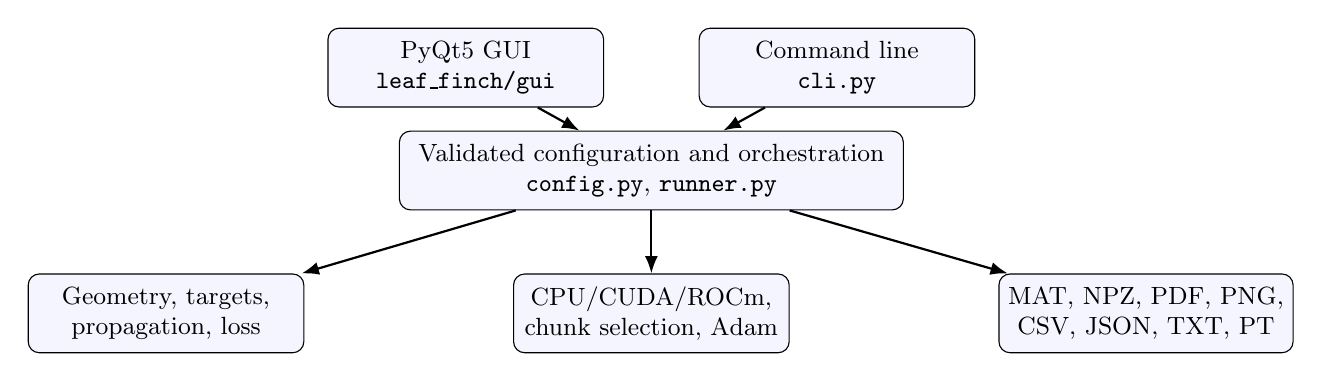
\begin{tikzpicture}[font=\small, node distance=8mm and 12mm,
box/.style={draw,rounded corners,minimum width=35mm,minimum height=10mm,align=center,fill=blue!4},
arrow/.style={-{Latex[length=2.2mm]},thick}]
\node[box] (gui) {PyQt5 GUI\\\texttt{leaf\_finch/gui}};
\node[box,right=of gui] (cli) {Command line\\\texttt{cli.py}};
\node[box,below=of $(gui)!0.5!(cli)$,minimum width=64mm] (runner) {Validated configuration and orchestration\\\texttt{config.py}, \texttt{runner.py}};
\node[box,below left=of runner] (physics) {Geometry, targets,\\propagation, loss};
\node[box,below=of runner] (runtime) {CPU/CUDA/ROCm,\\chunk selection, Adam};
\node[box,below right=of runner] (output) {MAT, NPZ, PDF, PNG,\\CSV, JSON, TXT, PT};
\draw[arrow] (gui) -- (runner);
\draw[arrow] (cli) -- (runner);
\draw[arrow] (runner) -- (physics);
\draw[arrow] (runner) -- (runtime);
\draw[arrow] (runner) -- (output);
\end{tikzpicture}
\caption{Main architectural layers. The GUI and CLI use the same numerical and output paths.}
\label{fig:architecture}
\end{figure}

The main package modules are summarized in \cref{tab:modules}.
\begin{table}[H]
\centering
\caption{Package modules.}
\label{tab:modules}
\begin{tabularx}{\textwidth}{@{}lX@{}}
\toprule
Module & Responsibility \\
\midrule
\texttt{geometry.py} & DMD coordinates, polygonal aperture, oblique plane, disk sampling. \\
\texttt{propagation.py} & Rayleigh--Sommerfeld blocks, incident wave, Fresnel FFT propagation. \\
\texttt{targets.py} & Target modes, apodization, FZP focal-power correction. \\
\texttt{optimization.py} & Straight-through masks, loss, OOM retry, deterministic FZP. \\
\texttt{adam.py} & Adam update specialized for the single logits tensor. \\
\texttt{backend.py} & Accelerator discovery and automatic chunk sizing. \\
\texttt{reconstruction.py} & Complex field reconstruction on a regular observation grid. \\
\texttt{training\_state.py} & Portable checkpoint save/load and validation. \\
\texttt{io.py} & Patterns, convergence, reconstructions, and metadata. \\
\texttt{runner.py} & End-to-end simulation sequence. \\
\bottomrule
\end{tabularx}
\end{table}

\section{Coordinate system and observation geometry}
\subsection{DMD sampling}
For a DMD of $N_x\times N_y$ pixels and pitch $p$, pixel-center coordinates are
\begin{align}
 x_i &= \left(i-\frac{N_x-1}{2}\right)p, && i=0,\ldots,N_x-1,\\
 y_j &= \left(j-\frac{N_y-1}{2}\right)p, && j=0,\ldots,N_y-1,
\end{align}
with source locations
\begin{equation}
 \vect r_m=(x_i,y_j,0),\qquad m=jN_x+i,
\end{equation}
and elementary area $\Delta A=p^2$. The DMD normal points in the positive $z$ direction.

The optional aperture is the largest even-sided regular polygon that fits inside the DMD rectangle. If $a$ is its apothem and $\alpha_l$ are outward-normal angles, pixel $m$ is active when
\begin{equation}
 x_m\cos\alpha_l+y_m\sin\alpha_l\leq a
 \quad\text{for every side }l.
\end{equation}
Disabling the aperture activates all pixels.

\subsection{Oblique observation plane}
The user supplies two direction angles, $\theta_x$ and $\theta_y$. The unit direction from the DMD center is
\begin{equation}
 \vect n=\left(\sin\theta_x,\;\sin\theta_y,\;\sqrt{1-\sin^2\theta_x-\sin^2\theta_y}\right),
 \label{eq:n}
\end{equation}
which requires $\sin^2\theta_x+\sin^2\theta_y<1$. For axial distance $L$, the center of the target disk is
\begin{equation}
 \boxed{\vect c=L\vect n}.\label{eq:center}
\end{equation}
Two orthonormal in-plane vectors $\vect e_1$ and $\vect e_2$ satisfy $\vect e_1\cdot\vect n=\vect e_2\cdot\vect n=0$. A point in the target plane is
\begin{equation}
 \vect r(\rho,\vartheta)=\vect c+\rho\cos\vartheta\,\vect e_1+\rho\sin\vartheta\,\vect e_2,
 \qquad 0\leq\rho\leq\Rdisk,
 \label{eq:plane-point}
\end{equation}
where
\begin{equation}
 \Rdisk=L\tan\theta_{\mathrm{disk}}.
\end{equation}

\begin{figure}[H]
\centering
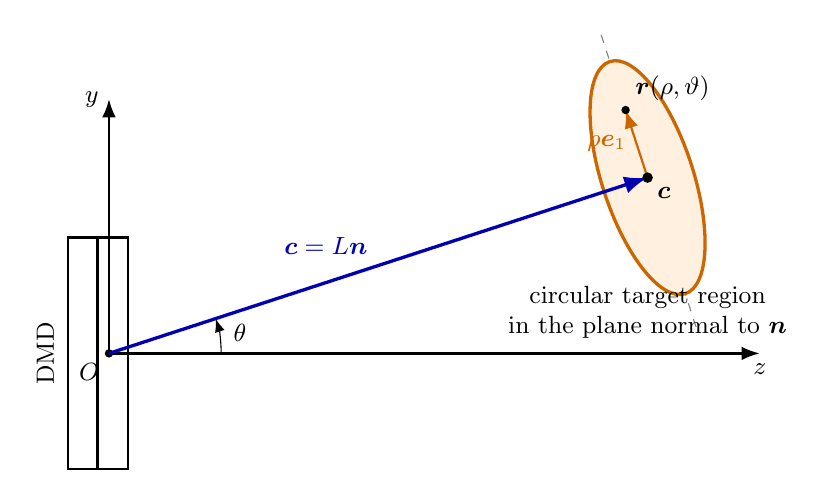
\begin{tikzpicture}[scale=0.95,>=Latex,font=\small]
  \coordinate (O) at (0,0);
  \coordinate (C) at (7.2,2.35);
  \draw[very thick] (-0.15,-1.55) -- (-0.15,1.55);
  \draw[thick] (-0.55,-1.55) rectangle (0.25,1.55);
  \node[rotate=90] at (-0.85,0) {DMD};
  \draw[->,thick] (O) -- (8.7,0) node[below] {$z$};
  \draw[->,thick] (O) -- (0,3.4) node[left] {$y$};
  \fill (O) circle (1.6pt) node[below left] {$O$};
  \coordinate (Q) at ($(C)+(108:0.95)$);
  \draw[dashed,gray] ($(C)+(288:2.1)$) -- ($(C)+(108:2.1)$);
  \node[ellipse,draw=orange!80!black,fill=orange!12,very thick,
    minimum width=31mm,minimum height=11.6mm,rotate=108,inner sep=0pt]
    at (C) {};
  \draw[->,very thick,blue!70!black] (O) -- (C)
    node[midway,above left] {$\vect c=L\vect n$};
  \draw[->,thick,orange!80!black] (C) -- (Q)
    node[midway,left] {$\rho\vect e_1$};
  \fill (Q) circle (1.6pt) node[above right] {$\vect r(\rho,\vartheta)$};
  \fill (C) circle (2pt) node[below right] {$\vect c$};
  \node[align=center] at (7.2,0.55)
    {circular target region\\in the plane normal to $\vect n$};
  \draw[->] (1.5,0) arc[start angle=0,end angle=18,radius=1.5];
  \node at (1.75,0.27) {$\theta$};
\end{tikzpicture}
\caption{Observation geometry. The circular target region lies in the plane normal to $\vect n$ and is centered exactly at $\vect c=L\vect n$. The implementation uses the two direction parameters in \cref{eq:n}.}
\label{fig:geometry}
\end{figure}

\subsection{Random disk sampling}
Each epoch samples $K$ new points. For independent $u\sim U(0,1)$ and $\vartheta\sim U(0,2\pi)$,
\begin{equation}
 \rho=\Rdisk\left[f u+(1-f)\sqrt{u}\right],\qquad 0\leq f\leq1.
 \label{eq:sampling}
\end{equation}
The setting $f=0$ gives uniform probability per unit area; $f=1$ gives a uniform radial coordinate. Intermediate values interpolate between the two distributions.

Optional DMD-coordinate jitter perturbs active source positions independently:
\begin{equation}
 \delta x_m,\delta y_m\sim U(-\eta p,\eta p),\qquad 0\leq\eta\leq\tfrac12.
\end{equation}
Thus $\eta=0.5$ samples the full interval $[-p/2,p/2]$.

\section{Incident field and Rayleigh--Sommerfeld propagation}
\subsection{Incident field}
A plane wave is selected with $z_i=\infty$. For finite incident wavefront radius $z_i$, the DMD illumination is
\begin{equation}
 U_{\mathrm{inc}}(x_m,y_m)=\exp\!\left[\ii\frac{k}{2z_i}(x_m^2+y_m^2)\right],
 \qquad k=\frac{2\pi}{\lambda}.
 \label{eq:incident}
\end{equation}
A spatially constant phase is omitted. Positive $z_i$ represents a divergent wave at the DMD.

\subsection{Discretized propagation}
For observation point $\vect r_q$ and source pixel $\vect r_m$, define
\begin{equation}
 \vect d_{qm}=\vect r_q-\vect r_m,\qquad R_{qm}=\lVert\vect d_{qm}\rVert,
 \qquad \cos\gamma_{qm}=\frac{d_{qm,z}}{R_{qm}}.
\end{equation}
For binary transmission $b_{nm}\in\{0,1\}$ of pattern $n$, the implemented first Rayleigh--Sommerfeld form is
\begin{equation}
 E_{qn}=\sum_{m=1}^{M} b_{nm}U_{\mathrm{inc},m}
 \frac{\cos\gamma_{qm}}{\ii\lambda R_{qm}}
 \exp(\ii kR_{qm})\left(1-\frac{1}{\ii kR_{qm}}\right)\Delta A.
 \label{eq:rs}
\end{equation}
The complex kernel is evaluated with real sine and cosine operations. The full $K\times M$ propagation matrix is never stored. Instead, active DMD pixels are partitioned into chunks $\mathcal C_j$:
\begin{equation}
 E_{qn}=\sum_j E_{qn}^{(\mathcal C_j)}.
\end{equation}
During optimization, a custom autograd recomputation function avoids retaining all block intermediates until backward propagation.

\section{Target modes}
Let $\phi_n=2\pi n/N$ and let $W(\rho)$ be the optional raised-cosine edge window. For edge width $w$, the window equals one for $\rho\leq\Rdisk-w$ and smoothly decreases to zero over the outer annulus.

\subsection{Quadratic cosine target}
For nonzero distance parameter $d$,
\begin{equation}
 T_n^{(\mathrm{cos})}(\rho)=W(\rho)
 \cos\!\left(\frac{k\rho^2}{2d}-\frac{\phi_n}{2}\right).
 \label{eq:cos-target}
\end{equation}

\subsection{Spherical-wave target}
The spherical target retains the exact radial distance to an axial point displaced by $d$:
\begin{equation}
 T_n^{(\mathrm{sph})}(\rho)=W(\rho)
 \frac{\cos\!\left(k\sqrt{\rho^2+d^2}-\frac{\phi_n}{2}\right)}{\sqrt{\rho^2+d^2}}.
 \label{eq:sph-target}
\end{equation}

\subsection{Siemens-star target}
For $S$ angular periods and pattern-dependent rotation $\beta_n$,
\begin{equation}
 B_n(\vartheta)=\mathbf 1\!\left[\cos\big(S(\vartheta-\beta_n)\big)\geq0\right],
\end{equation}
\begin{equation}
 T_n^{(\mathrm{Siemens})}(\rho,\vartheta)=W(\rho)
 \left[T_{\min}+(T_{\max}-T_{\min})B_n(\vartheta)\right].
\end{equation}
If the rotation step is not specified, the default is $180^\circ/(SN)$.

\subsection{Deterministic two-lens FZP}
The FZP mode skips gradient optimization. Its effective focal distances are $f_{\pm}^{\mathrm{eff}}=L\pm d$. For a finite incident wavefront radius, the physical lens focal length is corrected by
\begin{equation}
 \frac{1}{f_{\pm}}=\frac{1}{f_{\pm}^{\mathrm{eff}}}+\frac{1}{z_i}.
\end{equation}
The pre-threshold complex field is
\begin{equation}
 A_n(x,y)=\left[
 e^{\ii\phi_n}e^{-\ii k(x^2+y^2)/(2f_+)}+
 e^{-\ii k(x^2+y^2)/(2f_-)}
 \right]e^{\ii k(xn_x+yn_y)},
\end{equation}
where the second lens term is omitted when the two effective distances coincide. The binary mask is $b_n=\mathbf 1[\operatorname{Re}A_n\geq0]$.

\section{Binary relaxation and loss function}
\subsection{Straight-through binary estimator}
Each active DMD pixel has a real logit $\ell_{nm}$. At epoch $t$, the soft transmission is
\begin{equation}
 s_{nm}=\sigma\!\left(\frac{\ell_{nm}}{\tau_t}\right),
\end{equation}
with exponentially decreasing temperature
\begin{equation}
 \tau_t=\tau_0\left(\frac{\tau_1}{\tau_0}\right)^{t/(T-1)}.
\end{equation}
The forward pass uses
\begin{equation}
 b_{nm}=\mathbf 1[s_{nm}\geq 1/2],
\end{equation}
but the backward pass uses the derivative of $s_{nm}$. In stop-gradient notation,
\begin{equation}
 \widetilde b_{nm}=b_{nm}-\operatorname{sg}(s_{nm})+s_{nm}.
 \label{eq:ste}
\end{equation}

\subsection{Phase-insensitive modal correlation}
The targets $T_{qn}$ are real. Define
\begin{equation}
 c_n=\sum_{q=1}^{K} E_{qn}T_{qn},\qquad
 P_{E,n}=\sum_q |E_{qn}|^2,\qquad
 P_{T,n}=\sum_q T_{qn}^2.
\end{equation}
The normalized shape score is
\begin{equation}
 S_n=\frac{|c_n|}{\sqrt{P_{E,n}P_{T,n}}},\qquad 0\leq S_n\leq1,
\end{equation}
and the target-mode power is
\begin{equation}
 Q_n=\frac{|c_n|^2}{P_{T,n}}.
\end{equation}
Because $|c_n|$ is used, the criterion is insensitive to one global phase per pattern. There is no independent phase-loss term for the real targets.

The two data terms are
\begin{align}
 L_{\mathrm{shape}}&=-\frac1N\sum_{n=0}^{N-1}S_n,\\
 L_{\mathrm{power}}&=-\frac1N\sum_{n=0}^{N-1}\log(1+Q_n),
\end{align}
and
\begin{equation}
 L_{\mathrm{data}}=w_{\mathrm{shape}}L_{\mathrm{shape}}+
 w_{\mathrm{power}}L_{\mathrm{power}}.
\end{equation}

\subsection{Binarization penalty and total loss}
The relaxation penalty is
\begin{equation}
 L_{\mathrm{bin}}=\frac{1}{NM}\sum_{n,m}s_{nm}(1-s_{nm}),
 \qquad 0\leq L_{\mathrm{bin}}\leq\frac14.
\end{equation}
The optimized loss is
\begin{equation}
 \boxed{L_{\mathrm{total}}=L_{\mathrm{data}}+w_{\mathrm{bin}}L_{\mathrm{bin}}.}
 \label{eq:total-loss}
\end{equation}
With the default $w_{\mathrm{bin}}=2\times10^{-4}$, the weighted binary term is at most $5\times10^{-5}$. It is therefore plotted in a separate symmetric-logarithmic panel together with the unweighted penalty.

\begin{figure}[H]
\centering
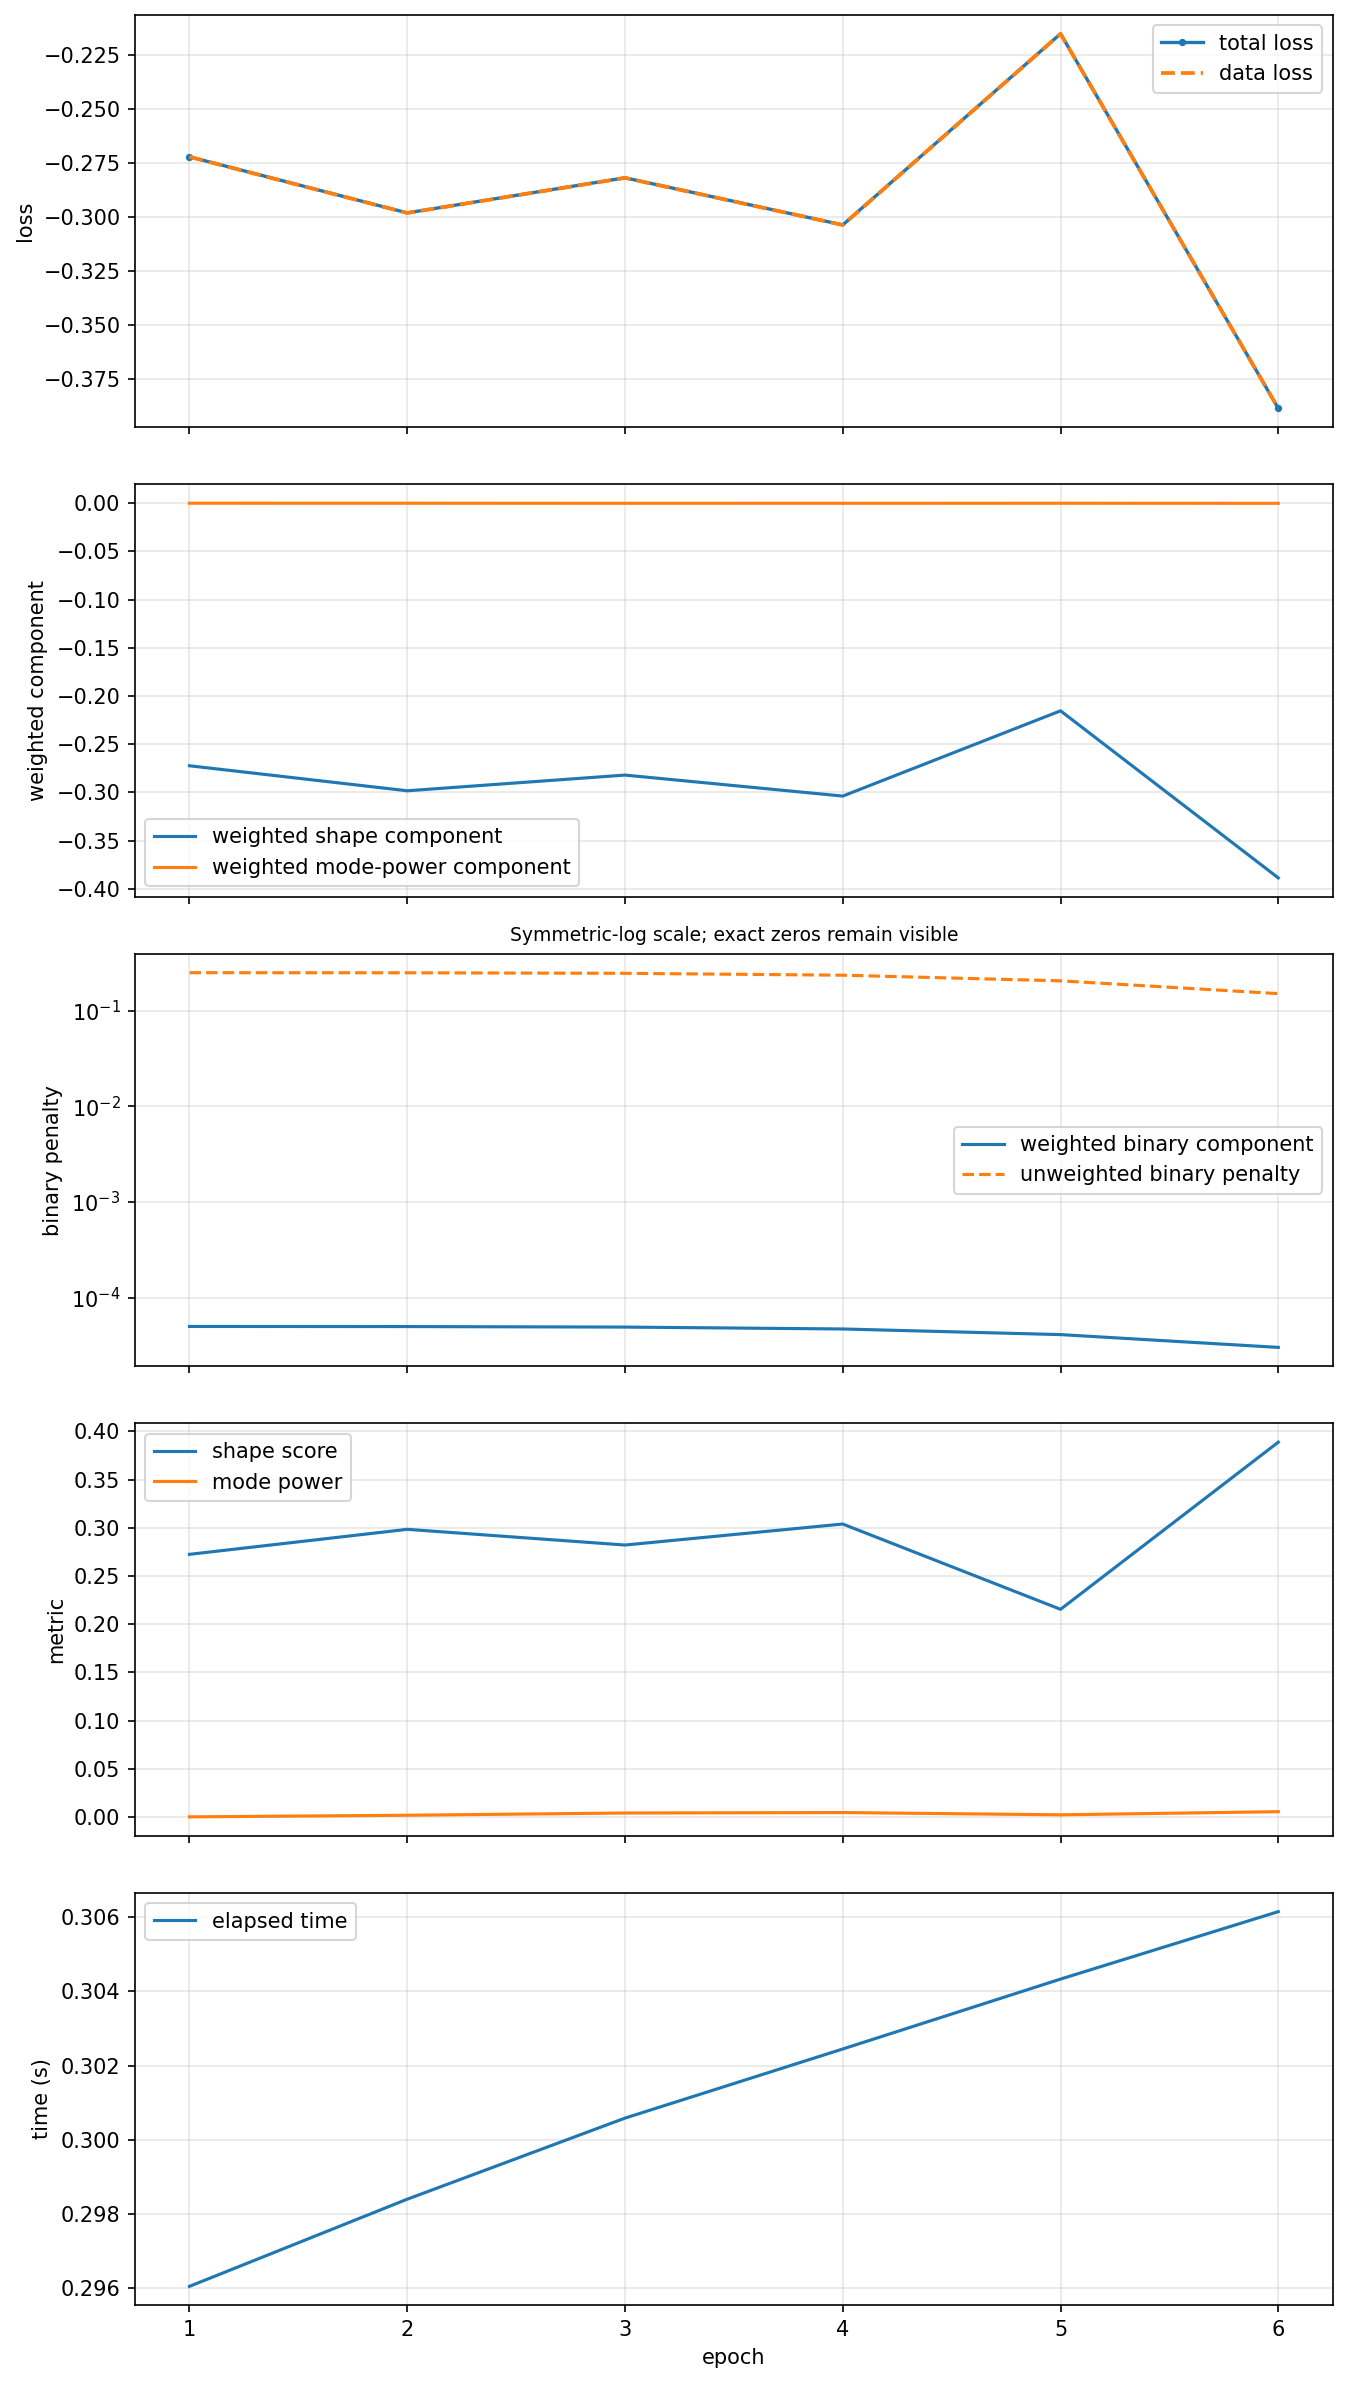
\includegraphics[width=0.86\textwidth]{assets/convergence_example.png}
\caption{Example convergence report. Total and data loss are separated from weighted physical components, while the weighted and unweighted binary penalties use a symmetric-logarithmic scale.}
\label{fig:loss}
\end{figure}

\section{Optimization algorithm and checkpoints}
The trainable logits are updated with Adam. For gradient $g_t=\nabla_{\ell}L_t$,
\begin{align}
 \vect m_t&=\beta_1\vect m_{t-1}+(1-\beta_1)\vect g_t,\\
 \vect v_t&=\beta_2\vect v_{t-1}+(1-\beta_2)\vect g_t^2,\\
 \widehat{\vect m}_t&=\frac{\vect m_t}{1-\beta_1^t},\qquad
 \widehat{\vect v}_t=\frac{\vect v_t}{1-\beta_2^t},\\
 \vect\ell_t&=\vect\ell_{t-1}-\alpha
 \frac{\widehat{\vect m}_t}{\sqrt{\widehat{\vect v}_t}+\epsilon_{\mathrm A}}.
\end{align}
\software{} uses a local implementation specialized for the single dense logits tensor. The update consists entirely of eager PyTorch operations and is portable across CPU, CUDA, and ROCm.

A training epoch performs the following operations:
\begin{enumerate}
  \item sample $K$ disk points and optionally jitter active DMD coordinates;
  \item evaluate all target patterns at the sampled points;
  \item convert logits to hard binary transmissions with \cref{eq:ste};
  \item propagate the fields in source-pixel chunks;
  \item evaluate \cref{eq:total-loss}, backpropagate, and update Adam;
  \item record all loss components, scores, temperature, chunk size, and time.
\end{enumerate}

\subsection{Stopping and resuming}
\textbf{Stop after current epoch} is checked only after the optimizer update and metric collection. It produces a coherent checkpoint and skips optional reconstruction. \textbf{Cancel immediately} is checked between propagation chunks; it may interrupt the current epoch and does not guarantee a new checkpoint.

A \texttt{model\_*.pt} checkpoint contains:
\begin{itemize}
  \item logits and aperture mask on CPU;
  \item Adam first and second moments, step count, and hyperparameters;
  \item completed and requested epoch counts;
  \item complete per-epoch history and elapsed time;
  \item random generator state and backend label;
  \item last temperature, chunk size, and full configuration.
\end{itemize}
The GUI and CLI can either continue the optimizer state or use only the stored logits as a fresh initialization.

\section{Accelerators, numerical precision, and memory management}
The performance-critical numerical path uses PyTorch on the selected device:
\begin{equation}
 \text{real geometry and logits: }\texttt{torch.float32},\qquad
 \text{complex fields: }\texttt{torch.complex64}.
\end{equation}
No automatic mixed precision or autocast is used. NumPy, SciPy, and Matplotlib are restricted to file export, plotting, and CPU-side interchange after numerical tensors have been computed.

ROCm builds of PyTorch expose AMD GPUs through the \texttt{torch.cuda} device API. Consequently, an AMD device can be represented internally as \texttt{cuda:0}; the backend is identified as ROCm from \texttt{torch.version.hip}.

For $K$ observation points and a chunk of $C$ active source pixels, dominant temporary arrays scale as
\begin{equation}
 \mathcal O(KC).
\end{equation}
The automatic selector reads currently free memory, reserves a user-defined margin, applies a memory fraction, and estimates safe source-pixel and reconstruction chunks. Training uses a more conservative estimate because autograd retains or recomputes additional intermediates. If an allocation still fails, source-pixel chunks are halved and retried; reconstruction can subsequently reduce its point chunk.

The oblique-plane basis is cached outside the epoch loop. Loss metrics are transferred to the host in one grouped operation per epoch. Reconstruction normally accumulates the complete complex field on the accelerator and transfers only final intensity and phase arrays to CPU.

\section{Reconstruction and FINCH hologram processing}
For a regular $G\times G$ grid in the observation plane, \software{} evaluates the complex field pattern by pattern using the same Rayleigh--Sommerfeld kernel. A global phase rotation makes the reconstructed complex field predominantly real without changing its intensity.

From phase-shifted intensity patterns $I_n(u,v)$, the complex FINCH hologram is formed as
\begin{equation}
 H(u,v)=\sum_{n=0}^{N-1}I_n(u,v)\exp\!\left(\ii\frac{2\pi n}{N}\right).
 \label{eq:hologram}
\end{equation}
Optional Fresnel reconstruction over distance $z_r$ uses convolution
\begin{equation}
 U_z=U_0*h_z,
\end{equation}
with impulse response
\begin{equation}
 h_z(x,y)=\frac{e^{\ii kz}}{\ii\lambda z}
 \exp\!\left[\ii\frac{k}{2z}(x^2+y^2)\right].
\end{equation}
The convolution is computed using zero-padded FFTs:
\begin{equation}
 U_z=\mathcal F^{-1}\!\left\{\mathcal F(U_0)\mathcal F(h_z)\right\}\Delta x\Delta y.
\end{equation}
Positive and negative distances can be exported to inspect the two conjugate reconstruction directions.

\section{Graphical user interface}
The GUI is launched with \texttt{leaf-finch-gui} or \texttt{python run\_gui.py}. Its three tabs are summarized in \cref{tab:gui}. The interface language can be switched at run time between English (default) and Polish. The translation applies to GUI widgets, labels, status messages, dialog titles, and plot annotations. File names, configuration keys, output-field names, source-code comments, and the distributed screenshots remain in English. The language selection is a presentation-only GUI setting and is not stored in \texttt{config.json} or model checkpoints.
\begin{table}[H]
\centering
\caption{GUI tabs.}
\label{tab:gui}
\begin{tabularx}{\textwidth}{@{}lX@{}}
\toprule
Tab & Main functions \\
\midrule
Parameters & Interface language, device and memory policy, DMD, observation geometry, illumination, target, loss weights, training, reconstruction, and output settings; configuration load/save; model load. \\
Simulation & Progress, textual log, three-panel live convergence plot, immediate cancellation, and graceful stop after the current epoch. \\
Results & Browse generated files, preview images and text data, open external files, and copy the saved model to a chosen location. \\
\bottomrule
\end{tabularx}
\end{table}

When a model is loaded, \textbf{Continue optimizer state, history, and epoch counter} interprets \textbf{Target total epochs} as the desired final epoch. If unchecked, only logits are loaded and the new run starts at epoch one with a fresh Adam state.


\subsection{Screenshot locations}
The screenshots distributed with the project show the default English interface and are intentionally not localized.

%The documentation source reserves the following figure locations for application screenshots. The distributed images are placeholders. Replace the corresponding PNG files in \texttt{docs/assets/screenshots/} without changing their filenames, then rebuild the document. A 16:9 image with a width of at least 1600 pixels is recommended.

\begin{figure}[H]
\centering
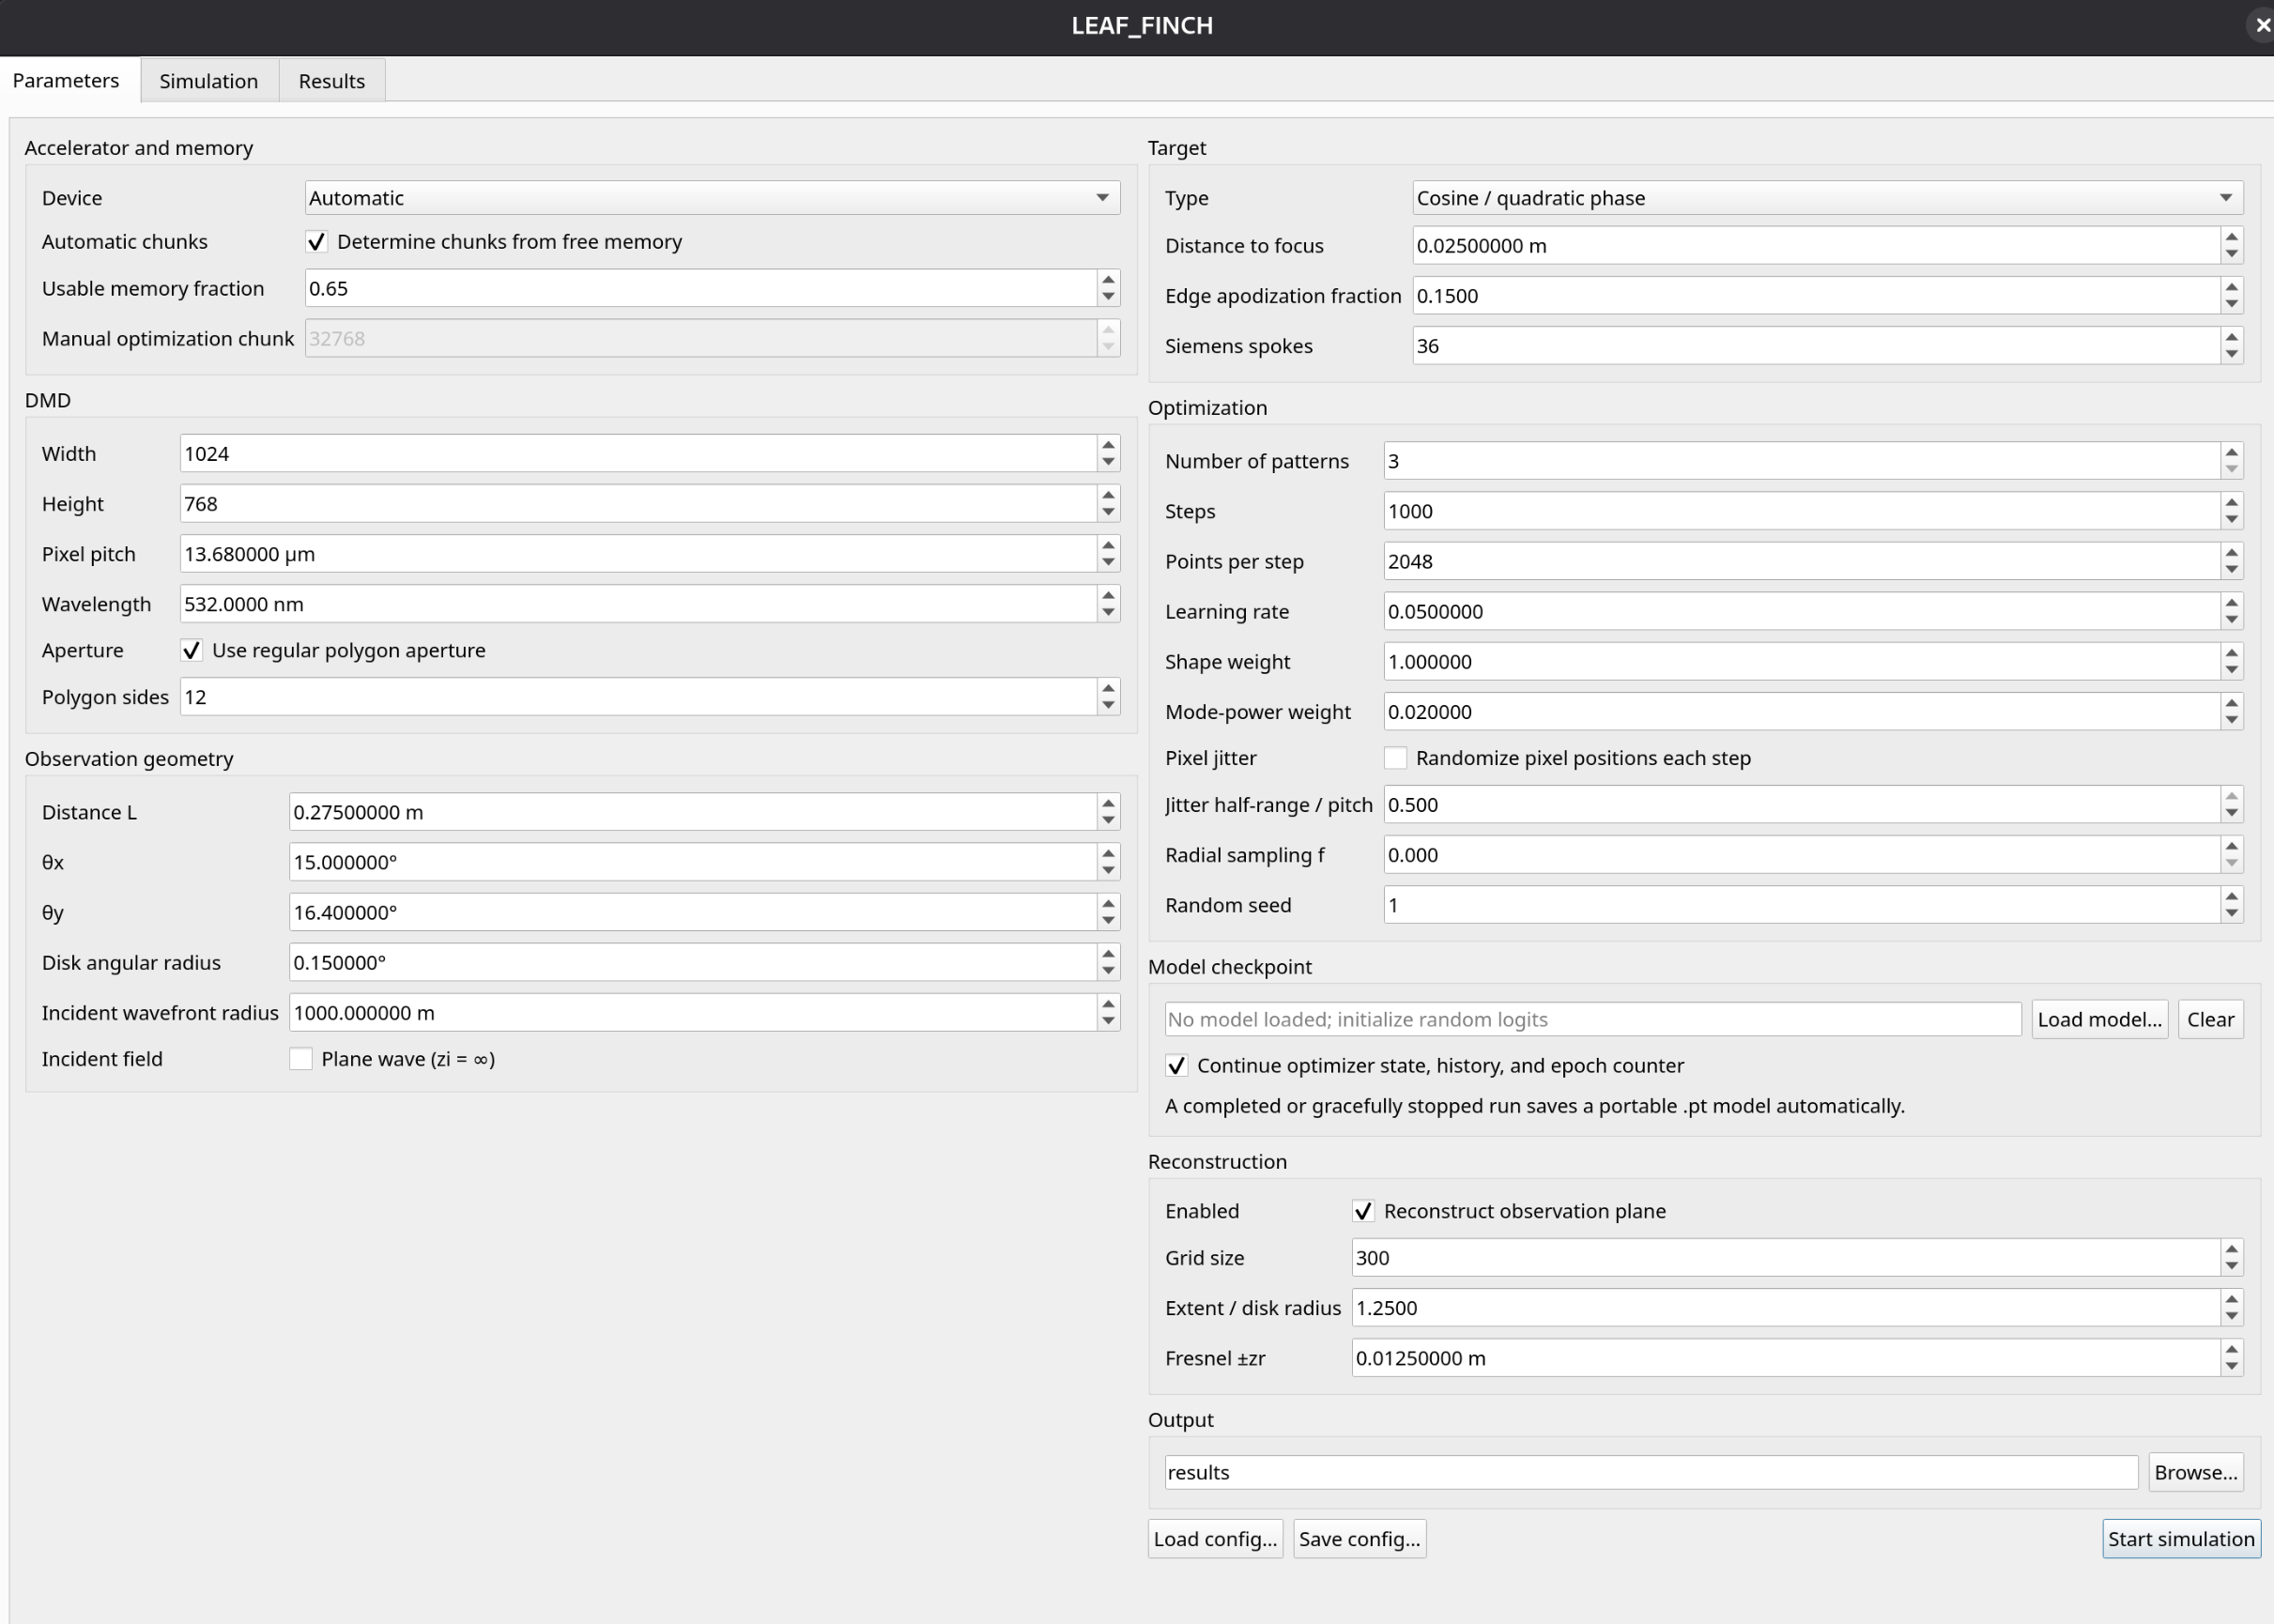
\includegraphics[width=0.92\textwidth]{assets/screenshots/main_window.png}
\caption{Parameters tab  showing device selection, DMD and observation geometry, target definition, optimization settings, reconstruction settings, and output controls.}
\label{fig:gui-parameters}
\end{figure}

\begin{figure}[H]
\centering
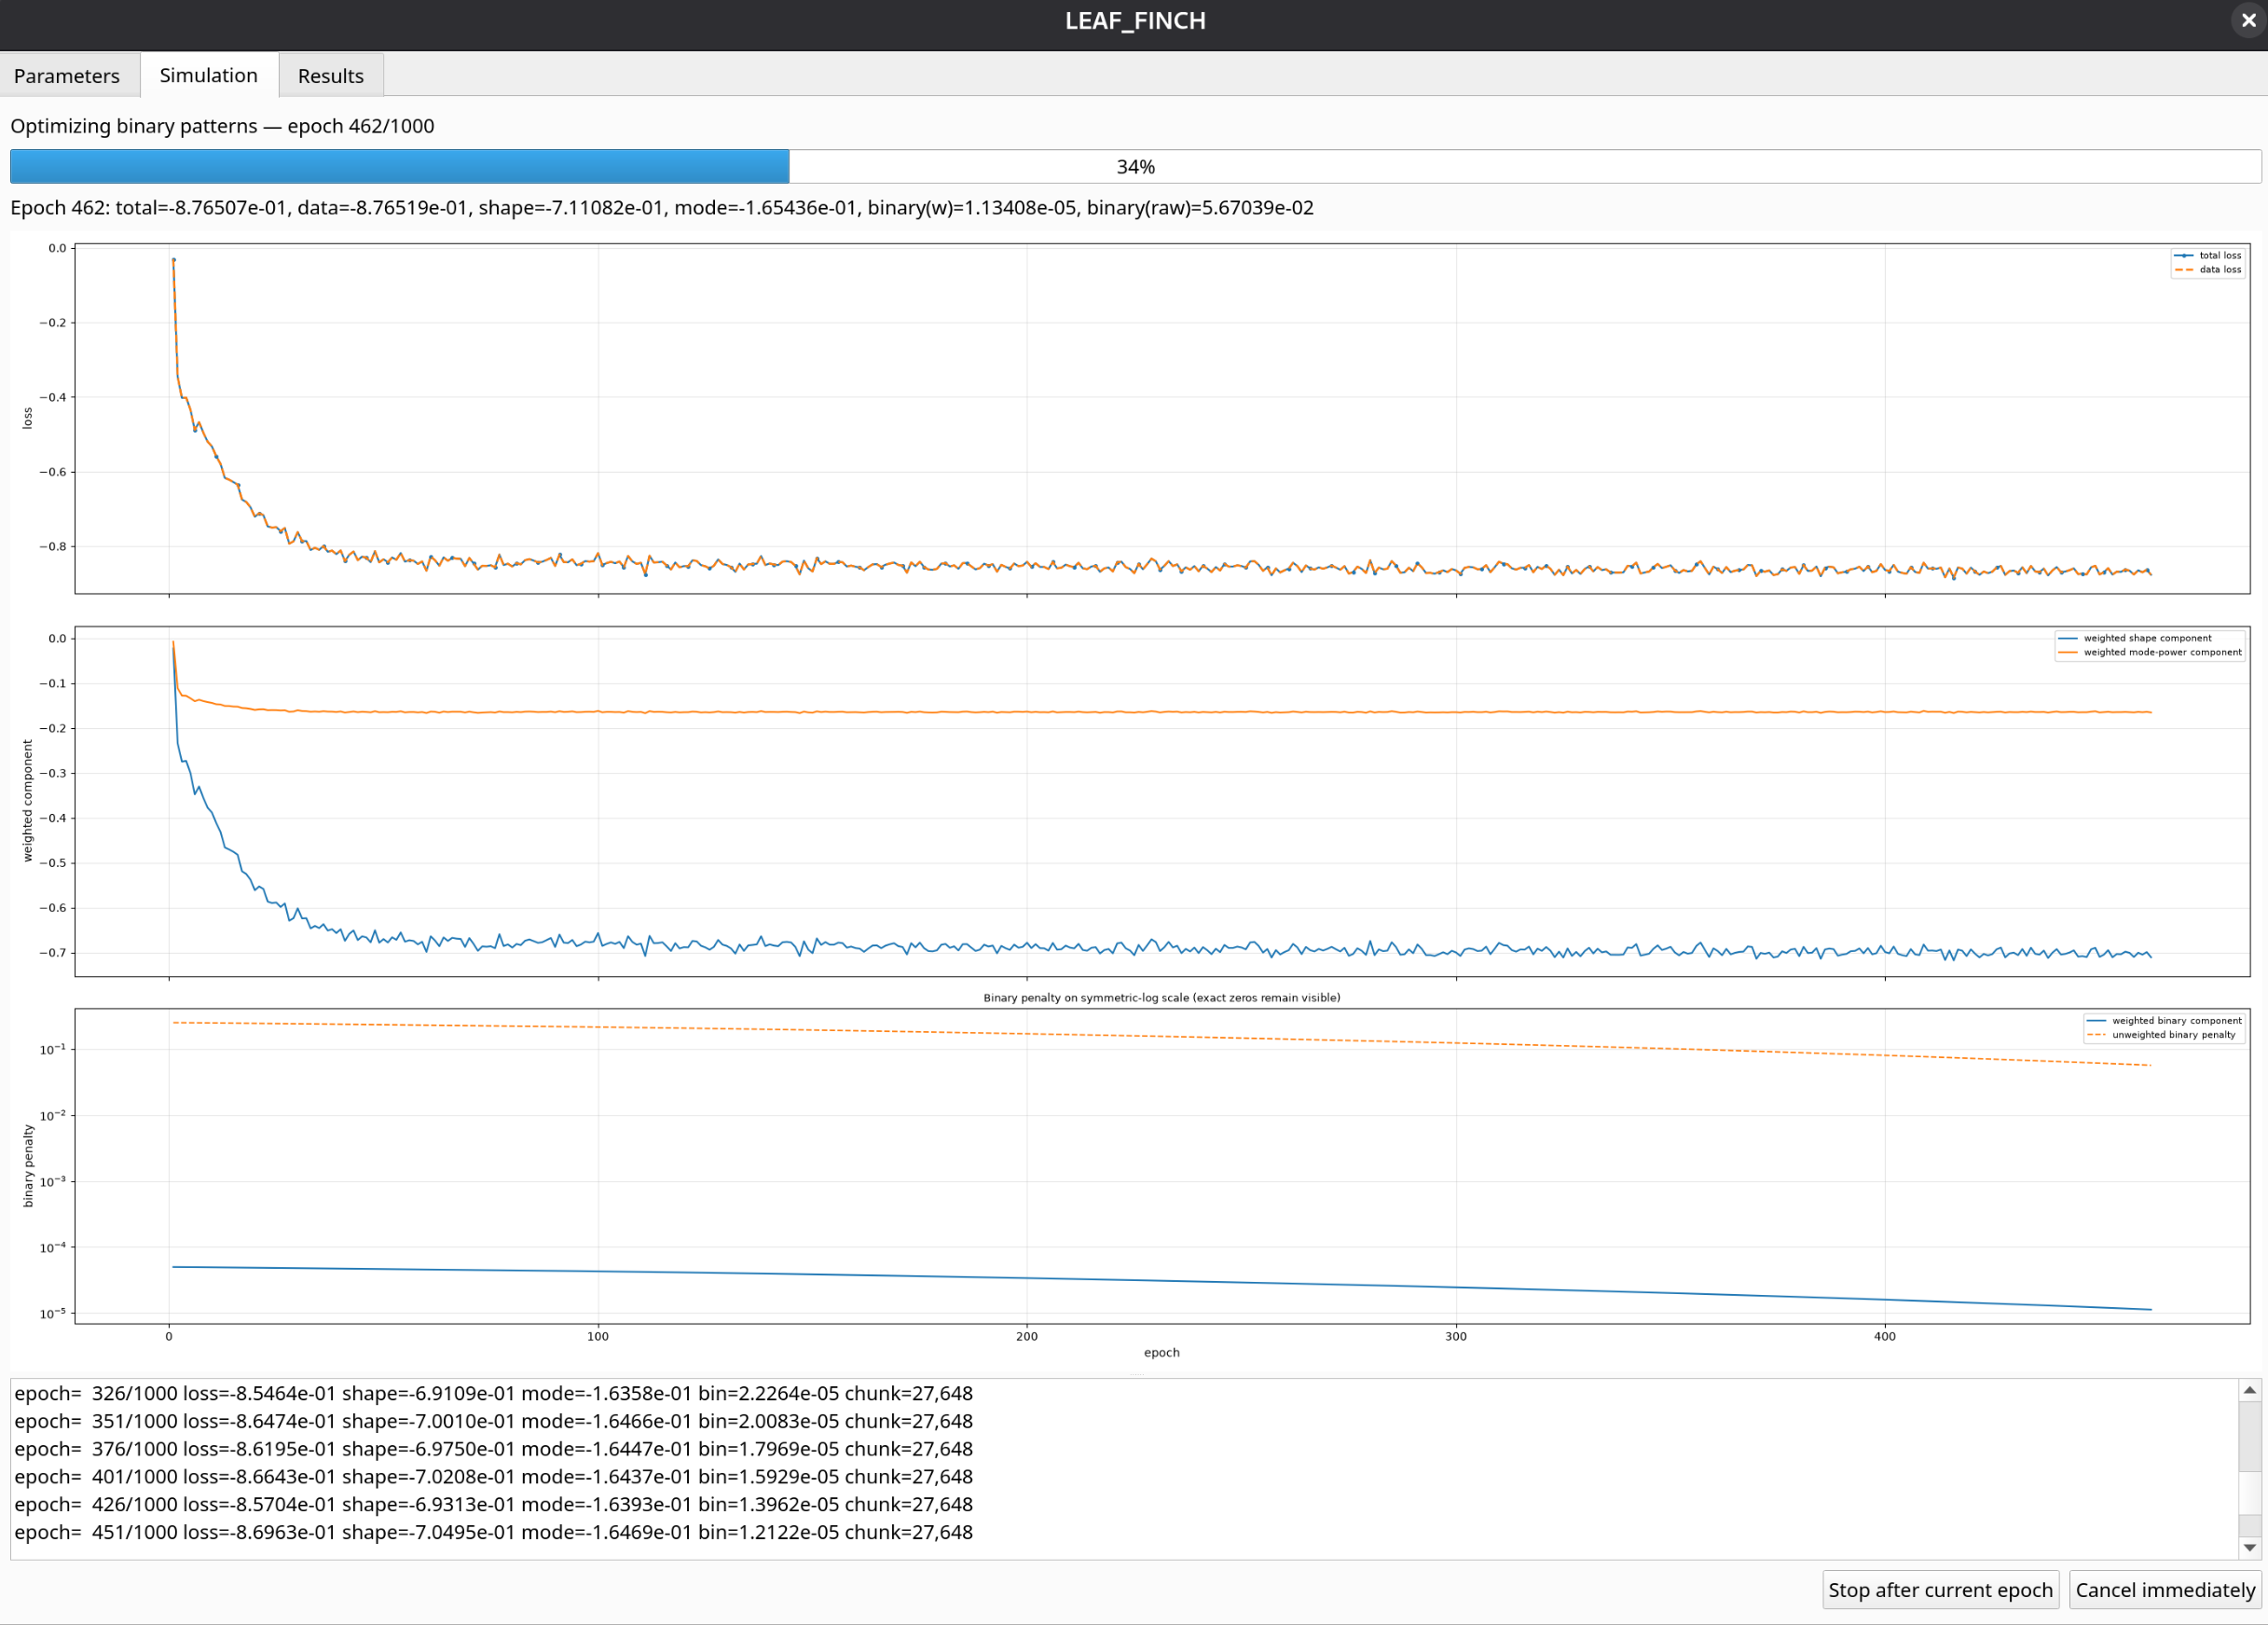
\includegraphics[width=0.92\textwidth]{assets/screenshots/live_optimization.png}
\caption{Simulation tab  showing optimization progress, the textual log, and the three-panel plot of the total loss and its components.}
\label{fig:gui-simulation}
\end{figure}

\begin{figure}[H]
\centering
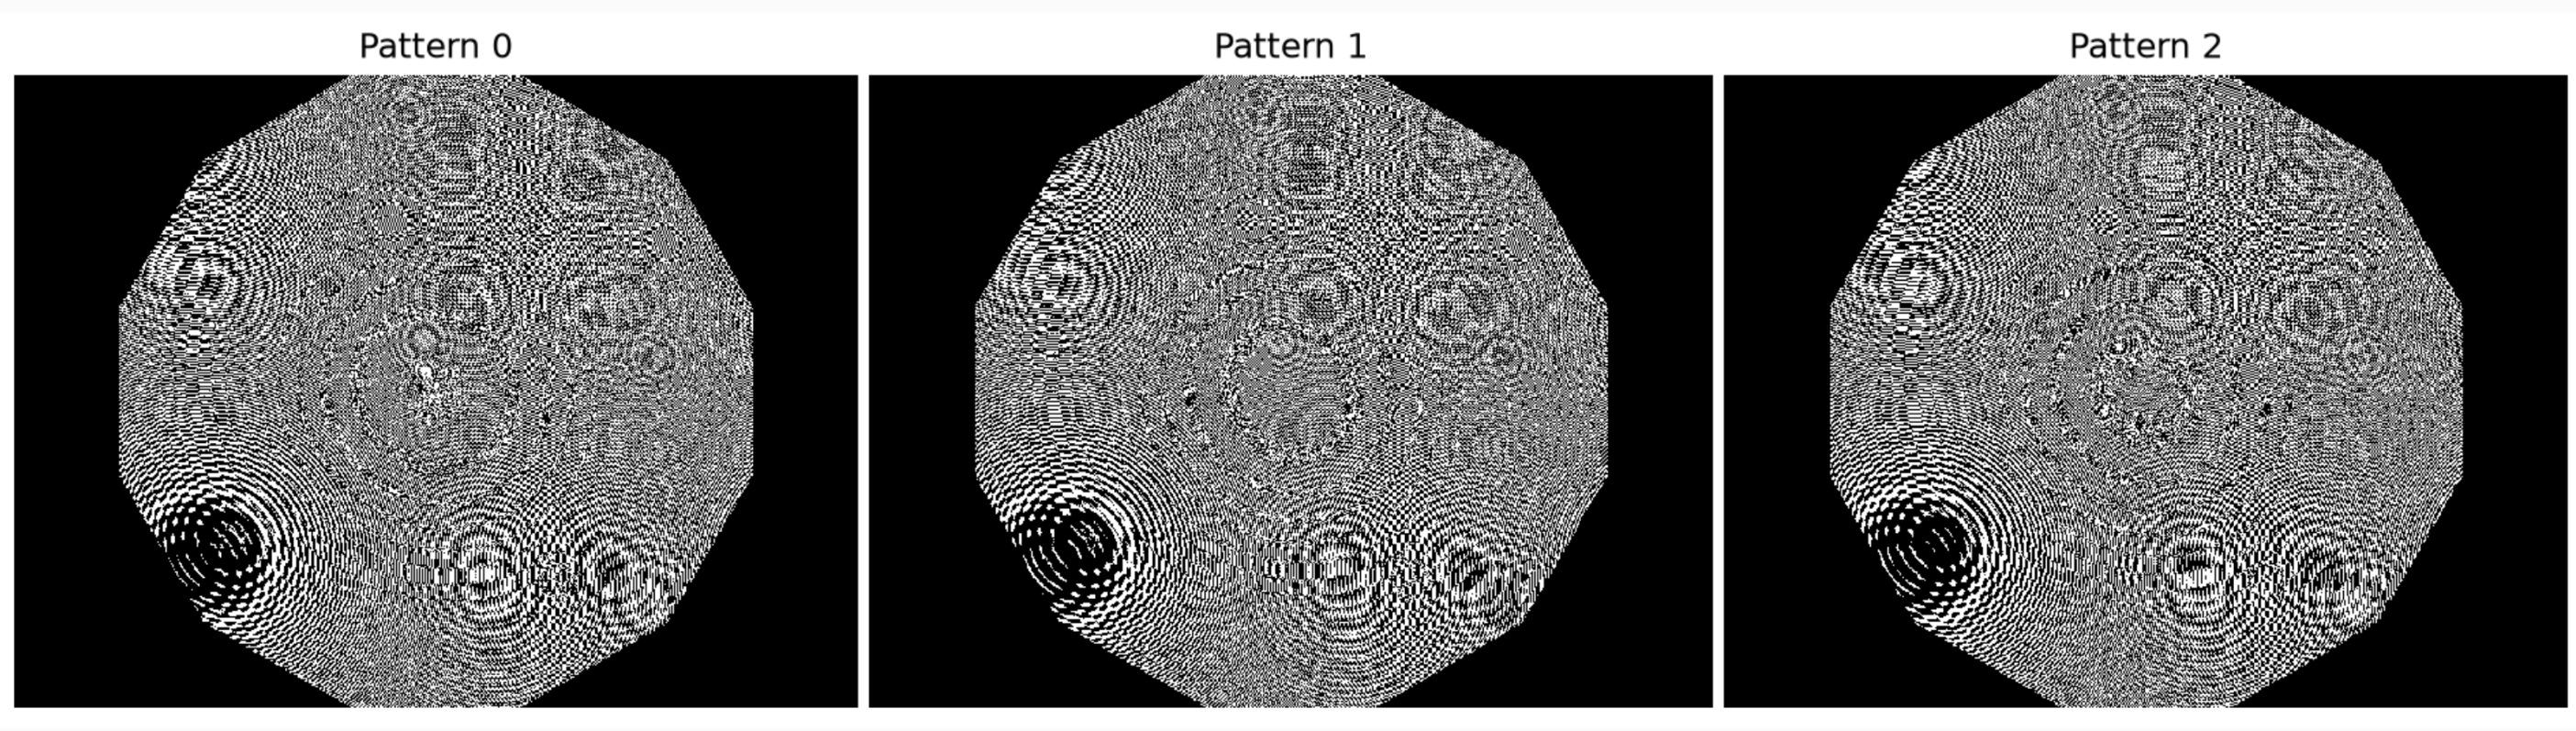
\includegraphics[width=0.92\textwidth]{assets/screenshots/results_browser.png}
\caption{Generated binary masks encoding 3 phase-shifted DMD patterns}
\label{fig:gui-results}
\end{figure}

\begin{figure}[H]
\centering
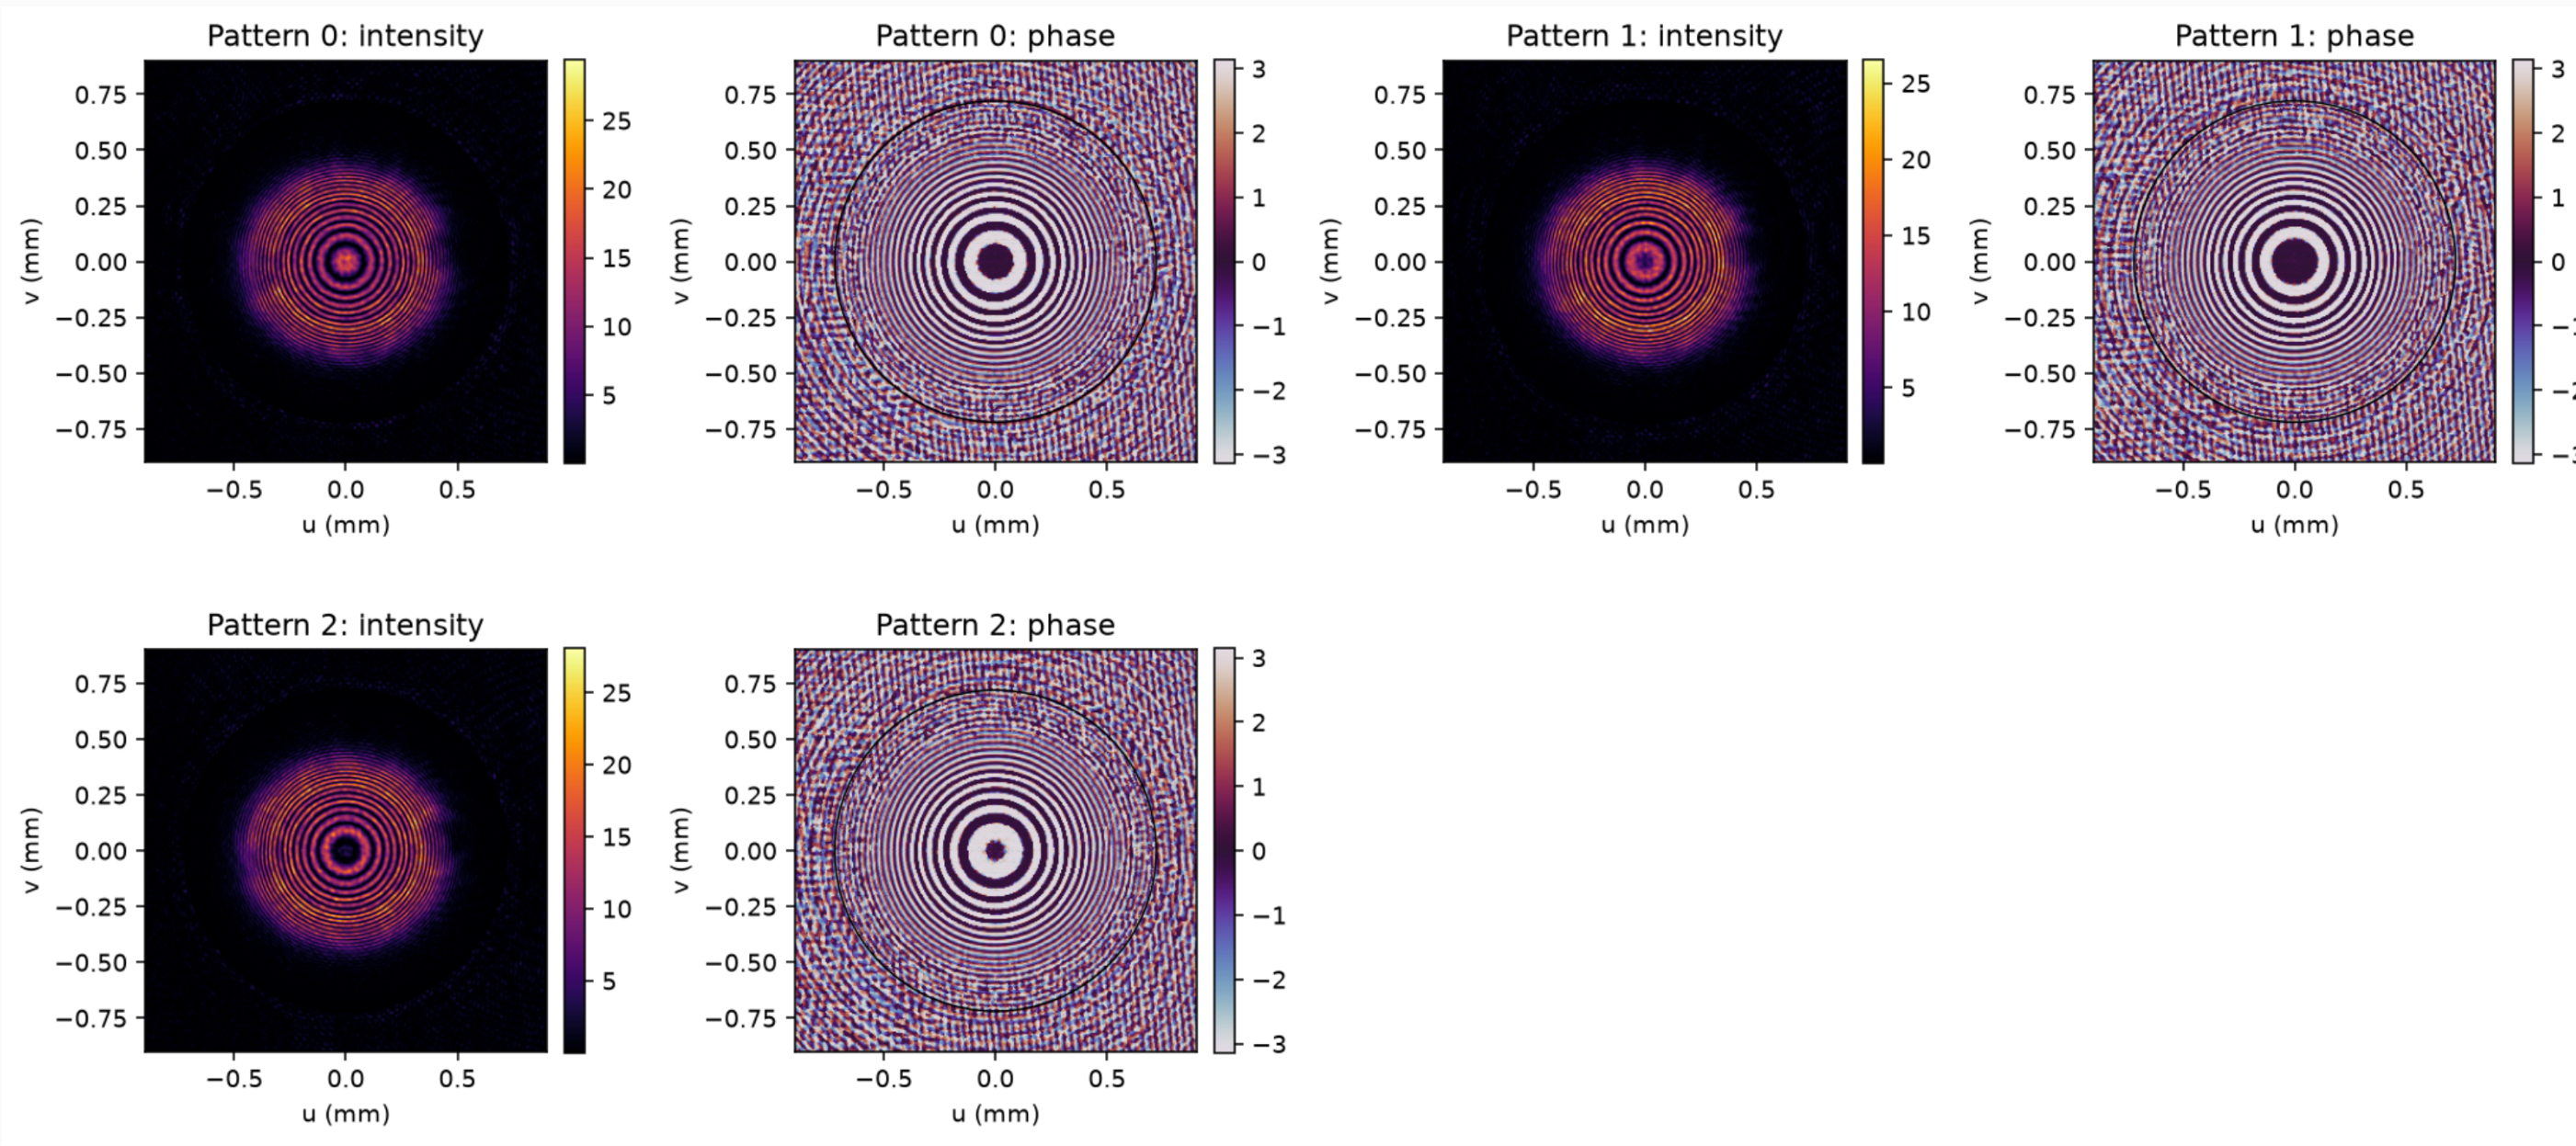
\includegraphics[width=0.92\textwidth]{assets/screenshots/results_reconstructed.png}
\caption{Reconstructed field (intensity and phase obtained at a circular off-axis target area; the phase-shifted target image together encode a complex-valued FINCH hologram)}
\label{fig:gui-reconstructed}
\end{figure}

\begin{figure}[H]
\centering
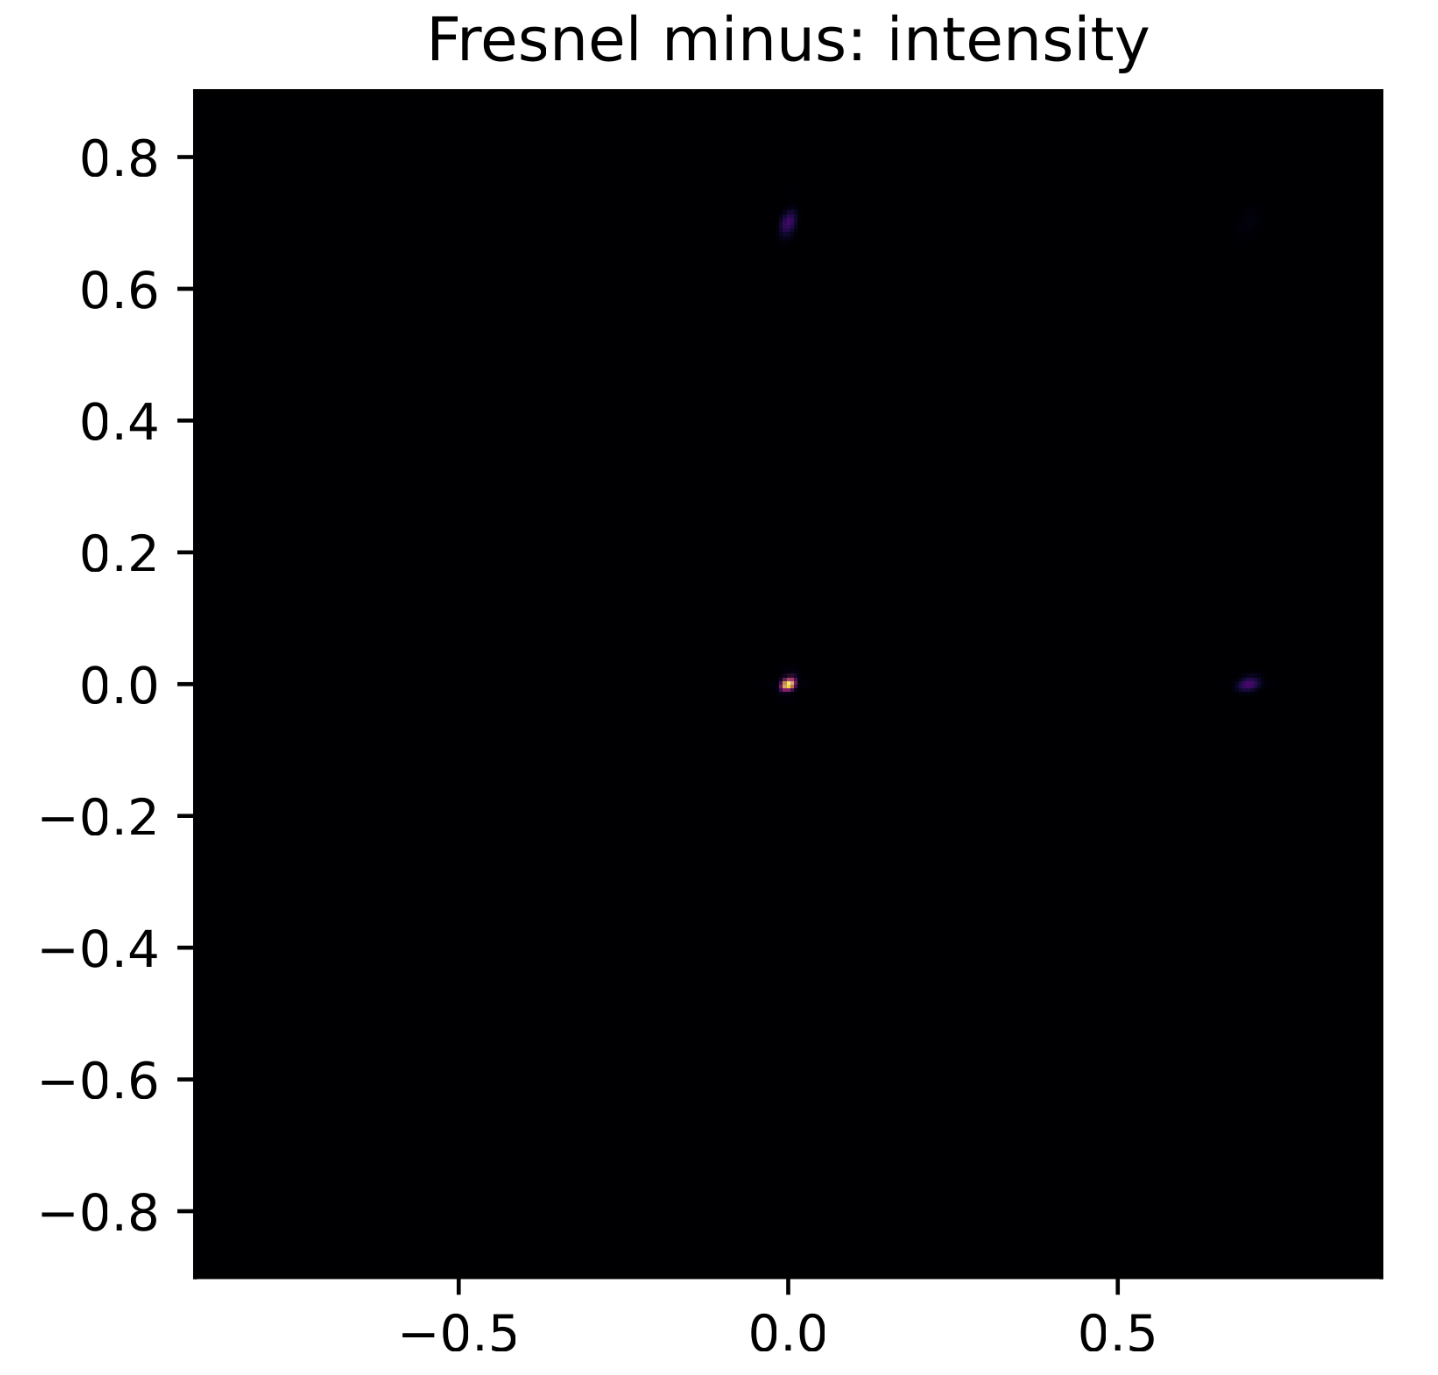
\includegraphics[width=0.92\textwidth]{assets/screenshots/finch_psf.png}
\caption{Reconstructed PSF of the complex FINCH hologram  (result of phase-shifted hologram reconstruction followed by Fresnel backpropagation)}
\label{fig:gui-psf}
\end{figure}


\section{Command-line interface}
Typical commands are:
\begin{lstlisting}[language=bash]
leaf-finch --list-devices
leaf-finch --write-default config.json
leaf-finch --config examples/default_config.json
leaf-finch --config config.json --model model_checkpoint.pt
leaf-finch --config config.json --model model_checkpoint.pt --restart-from-weights
\end{lstlisting}
The module form \texttt{python -m leaf\_finch} and direct launcher \texttt{python run\_cli.py} are equivalent.

\section{Configuration reference}
The JSON configuration contains the groups in \cref{tab:config}. Lengths are in metres and angles are in degrees unless indicated otherwise.
\begin{longtable}{@{}p{31mm}p{37mm}p{79mm}@{}}
\caption{Principal configuration fields.}\label{tab:config}\\
\toprule
Group & Field & Meaning \\
\midrule
\endfirsthead
\toprule
Group & Field & Meaning \\
\midrule
\endhead
\texttt{backend} & \texttt{device} & \texttt{auto}, \texttt{cpu}, \texttt{cuda:0}, or another discovered accelerator. \\
 & \texttt{auto\_batch} & Enable memory-based chunk selection. \\
 & \texttt{memory\_fraction} & Fraction of currently free memory available to the selector. \\
 & \texttt{reserve\_memory\_mb} & Additional memory margin. \\
\addlinespace
\texttt{dmd} & \texttt{nx}, \texttt{ny} & DMD dimensions; \texttt{nx} must be divisible by eight for packed output. \\
 & \texttt{pitch}, \texttt{wavelength} & Pixel pitch and wavelength. \\
 & \texttt{aperture\_sides} & Requested even-sided regular polygon. \\
 & \texttt{use\_aperture} & Use polygon or all DMD pixels. \\
\addlinespace
\texttt{plane\_angles} & \texttt{L} & Distance to disk center along $\vect n$. \\
 & \texttt{theta\_x\_deg}, \texttt{theta\_y\_deg} & Direction parameters in \cref{eq:n}. \\
 & \texttt{theta\_ring\_deg} & Disk angular radius. \\
\addlinespace
\texttt{incident} & \texttt{wavefront\_radius\_zi} & Incident wavefront radius; use the JSON string \texttt{"inf"} for a plane wave. \\
\addlinespace
\texttt{optimization} & \texttt{n\_patterns}, \texttt{n\_steps} & Number of phase-shifted masks and target total epochs. \\
 & \texttt{points\_per\_step} & Random disk samples per epoch. \\
 & \texttt{lr} & Adam learning rate. \\
 & \texttt{temperature\_start/end} & Straight-through sigmoid schedule. \\
 & \texttt{shape\_weight} & $w_{\mathrm{shape}}$. \\
 & \texttt{mode\_power\_weight} & $w_{\mathrm{power}}$. \\
 & \texttt{binarization\_weight} & $w_{\mathrm{bin}}$. \\
 & \texttt{dmd\_pixel\_jitter} & Enable randomized source coordinates. \\
 & \texttt{jitter\_fraction} & $\eta$ in units of pitch, limited to $[0,0.5]$. \\
 & \texttt{radial\_sampling\_f} & Sampling parameter $f$ in \cref{eq:sampling}. \\
\addlinespace
\texttt{target} & \texttt{target\_type} & \texttt{cosine}, \texttt{spherical}, \texttt{siemens}, or \texttt{fzp}. \\
 & \texttt{distance\_to\_focus} & Target parameter $d$. \\
 & \texttt{edge\_apodization\_*} & Raised-cosine outer annulus. \\
 & \texttt{siemens\_*} & Spokes, rotation, and low/high levels. \\
\addlinespace
\texttt{reconstruction} & \texttt{enabled}, \texttt{grid\_size} & Enable regular-grid reconstruction and choose resolution. \\
 & \texttt{distance}, \texttt{theta\_ring\_deg} & Optional reconstruction plane distance and radius. \\
 & \texttt{extent\_factor} & Grid half-width relative to disk radius. \\
 & \texttt{fresnel\_zr} & Optional positive/negative Fresnel propagation distance. \\
\addlinespace
\texttt{output} & \texttt{base\_dir} & Parent output directory. \\
 & \texttt{save\_convergence} & Save per-epoch report files. \\
 & \texttt{save\_reconstruction} & Save reconstructed fields. \\
\bottomrule
\end{longtable}

\section{Output files and reproducibility}
Every run writes the exact configuration and a metadata manifest. The principal files are:
\begin{itemize}
  \item \texttt{patterns\_*.mat}: packed $N\times N_y\times(N_x/8)$ \texttt{uint8} array named \texttt{Patterns}, with big-endian bit order;
  \item \texttt{patterns\_*.npz}: unpacked binary patterns;
  \item \texttt{convergence\_*}: complete per-epoch loss components, scores, temperature, time, and chunk size;
  \item \texttt{model\_*.pt}: resumable optimizer checkpoint;
  \item \texttt{reconstruction\_*.mat}: intensity, phase, local coordinates, complex hologram, and optional propagated fields;
  \item \texttt{run.json}: structured configuration, device, types, chunks, file paths, and status;
  \item \texttt{info.txt}: human-readable summary and final-epoch loss values.
\end{itemize}
For reproducibility, preserve \texttt{config.json}, \texttt{run.json}, the checkpoint, PyTorch version, backend version, GPU model, and random seed.

\section{Physical and numerical limitations}
\begin{itemize}
  \item Each DMD pixel is modeled as a uniform scalar source of area $p^2$. Mirror tilt, fill factor, polarization, wavelength-dependent reflectance, and micromirror diffraction are not modeled separately.
  \item The finite-radius incident field uses a quadratic phase. For strongly nonparaxial illumination, an exact spherical phase may be preferable.
  \item The target loss measures modal projection at Monte Carlo points rather than uniform error over a fixed dense grid.
  \item The target is real-valued and the loss is insensitive to a global phase for each pattern. It does not enforce an absolute output phase.
  \item Single precision is selected for speed and accelerator compatibility. Extremely large propagation distances, very small wavelengths, or severe cancellation may require a double-precision extension.
  \item Fresnel post-propagation is paraxial even though the DMD-to-oblique-plane propagation is Rayleigh--Sommerfeld.
  \item The program simulates masks and fields; hardware control and camera-in-the-loop calibration are outside version 1.0.
\end{itemize}

\section{Installation, tests, citation, and license}
Install a platform-appropriate PyTorch build first, then install the repository:
\begin{lstlisting}[language=bash]
python -m venv .venv
source .venv/bin/activate
# Install CPU/CUDA/ROCm PyTorch for this computer.
pip install -e .
python -m pytest
leaf-finch-gui
\end{lstlisting}
The repository includes a GitHub Actions workflow for CPU tests on supported Python versions.

If \software{} contributes to a publication, use the citation stored in \texttt{CITATION.cff} and \texttt{CITATION.bib}. The accompanying article is published in \emph{Optics Letters}:
\begin{quote}
Vijayakumar Anand, Rafał Stojek, and Rafał Kotyński, ``Learned binary amplitude mask designs for Fresnel incoherent correlation holography,'' \emph{Opt. Lett.} \textbf{51}, 4825--4828 (2026), \href{https://doi.org/10.1364/OL.609636}{https://doi.org/10.1364/OL.609636}.
\end{quote}
Project homepage: \url{https://github.com/rkotynski/leaf_finch}.

The software is distributed under the MIT License. The license permits use, modification, redistribution, sublicensing, and commercial use, subject to retention of the copyright and license notice. The software is provided without warranty.

\end{document}
